%<dscrpt>Géométrie plane.</dscrpt>
Dans un plan muni d'un rep{\`e}re orthonorm{\'e} $(O,\overrightarrow{i},\overrightarrow{j})$, on note $D_m$ la droite d'{\'e}quation $y=mx$ pour tout $m>0$.\newline
Soit $M$ un point du plan, $A$ est sa projection sur l'axe des $x$ et $B$ sa projection sur l'axe des $y$. Par $A$ et $B$ on m{\`e}ne les parall{\`e}les {\`a} $D_m$ qui coupent respectivement l'axe des $y$ en $A'$ et l'axe des $x$ en $B'$.\newline
On appelle $M'$ le point qui se projette en $A'$ et $B'$ sur les axes. On note $\mathcal{T}_m$ l'application du plan dans lui m{\^e}me qui {\`a} $M$ associe $M'$.
\begin{figure}[!h]
 \centering
 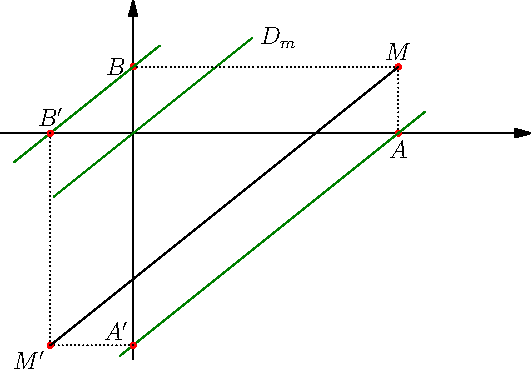
\includegraphics{Egep1_1.pdf}
\end{figure}

\begin{enumerate}
  \item Calculer les coordonn{\'e}es $(a',b')$ de $M'$ en fonction des coordonn{\'e}es $(a,b)$ de $M$. Montrer que $\mathcal{T}_m$ est bijective et calculer $\mathcal{T}_m ^{-1}$.

  \item Quand la droite $(M\mathcal{T}_m(M))$ est-elle d{\'e}finie? Montrer que sa direction est alors ind{\'e}pendante de $M$ et que le milieu $P$ de $[M\mathcal{T}_m(M)]$ d{\'e}crit une droite $\delta_m$ que l'on d{\'e}terminera.\newline
  Quelle est la nature de $\mathcal{T}_m$ ? Peut-elle {\^e}tre une sym{\'e}trie orthogonale ?

  \item Le r{\'e}el $m$ {\'e}tant fix{\'e}, on suppose que $M$ d{\'e}crit une droite passant par $O$.
    \begin{enumerate}
      \item Que peut-on dire de l'ensemble des droites $(AB)$ ?
      \item Que peut-on dire de l'ensemble des droites $(A'B')$ ?
    \end{enumerate}

  \item On suppose que $M$ est fix{\'e} et que $m$ d{\'e}crit l'ensemble des r{\'e}els strictement positifs.
    \begin{enumerate}
      \item D{\'e}terminer l'ensemble
      \[\mathcal{H}=\{\mathcal{T}_m(M), m>0\}\]
      \item On suppose que $M$ n'est pas situ{\'e} sur les axes. Montrer que la tangente en $\mathcal{T}_m(M)$ {\`a} $\mathcal{H}$ est l'image de la droite $(A'B')$ par une homoth{\'e}tie de centre $O$ que l'on pr{\'e}cisera.
    \end{enumerate}

 \end{enumerate}

 \index{symétrie axiale}
 \index{homothétie}
